\documentclass[a4paper,12pt]{article}
\usepackage{multirow}
\usepackage[icelandic]{babel}
\usepackage[T1]{fontenc}
\usepackage[utf8x]{inputenc}
\usepackage{graphicx}
\usepackage{fancyhdr}
\usepackage[top=1.4in, bottom=1.4in, left=1.2in, right=1.2in]{geometry}
\usepackage[T1]{fontenc}
\usepackage{textcomp}
\usepackage{gensymb}
\usepackage{pdflscape}
\usepackage[framed,numbered,autolinebreaks,useliterate]{mcode}\lstset{language=matlab} 
\lstset{inputencoding=latin1}
\usepackage{caption}
\usepackage{here}
\usepackage{amsmath} % or simply amstext
\newcommand{\angstrom}{\textup{\AA}}
\usepackage{subcaption}
\usepackage{url} 
%\usepackage[table]{xcolor}
\usepackage[version=3]{mhchem}
\usepackage{layout}
\usepackage[parfill]{parskip}
\usepackage{arydshln}
\pagestyle{fancy}
\lhead{}
\chead{}
\rhead{IÐN401G \\ Vor 2014}
\lfoot{Háskóli Íslands}
\cfoot{}
\rfoot{\thepage}
\renewcommand{\headrulewidth}{0.0pt}
\renewcommand{\footrulewidth}{0.0pt}

\begin{document}
\begin{titlepage}
\begin{center}
\begin{minipage}{0.4\textwidth}
\begin{flushleft} 
\vspace{10mm}
        \begin{figure}[H]
      
\includegraphics[width=0.4\linewidth]{HI_merki.jpg}
        \label{fig: logo}
        \end{figure}
\end{flushleft}
\end{minipage}
\begin{minipage}{0.4\textwidth}
\begin{flushright} \large
\textsc{Háskóli Íslands\\Verkfræðideild}
\end{flushright}
\end{minipage}

\vspace{4cm}



%
\includegraphics[width=0.15\textwidth]{HI_merki.jpg}\\[1cm]


{\textsc{\Large Aðgerðagreining}\\[0.5cm]}

\vspace{0.8cm}
% Title
\begin{center}
\rule{1\textwidth}{3pt}

{\textsc{ \LARGE \bfseries Bestun stundatöflu í stokkakerfi}} \\[0.4cm]



\rule{1\textwidth}{4pt}
\vspace{2cm}

\end{center}
\today

\vfill

\begin{minipage}{0.4\textwidth}
\begin{flushleft} 
\vspace{1cm}
\emph{Kennari:}\\
\textsc{Tómas Philip Rúnarsson}\\
\end{flushleft}
\end{minipage}
\begin{minipage}{0.4\textwidth}
\begin{flushright} 
\emph{Nemendur:}\\
Baldur Geir Gunnarsson\\
Einar Halldórsson\\
Gestur Hvannberg\\
Oddur Vilhjálmsson\\
Trausti Kouichi Ásgeirsson
\end{flushright}
\end{minipage}
% Bottom of the page
%{\large Vorönn, 2014}

\end{center}

\newpage
\thispagestyle{empty} \mbox{}
\vfill
%\begin{center}\textit{\thesisdedication}\end{center} \vspace*{5cm}
\vfill 
\thispagestyle{empty}
\cleardoublepage



\end{titlepage}

\title{Bestun stundatöflu í stokkakerfi}
\author{Baldur Geir Gunnarsson, Einar Halldórsson, Gestur Hvannberg,\\ Oddur Vilhjálmsson, Trausti Kouichi Ásgeirsson}
\maketitle

\section{Ágrip}
Verkfræði og náttúruvísindasvið Háskóla Íslands notast við stokkakerfi við stundatöflugerð. Samtals eru 7 stokkar á hverri önn og raða þarf áföngum niður á þá. Markmið okkar var að hanna stundatöflur fyrir allar annir í Eðlisfræði og kanna eiginlega þeirrar lausnar. Stokkarnir líta svona út í dag:

\begin{center}
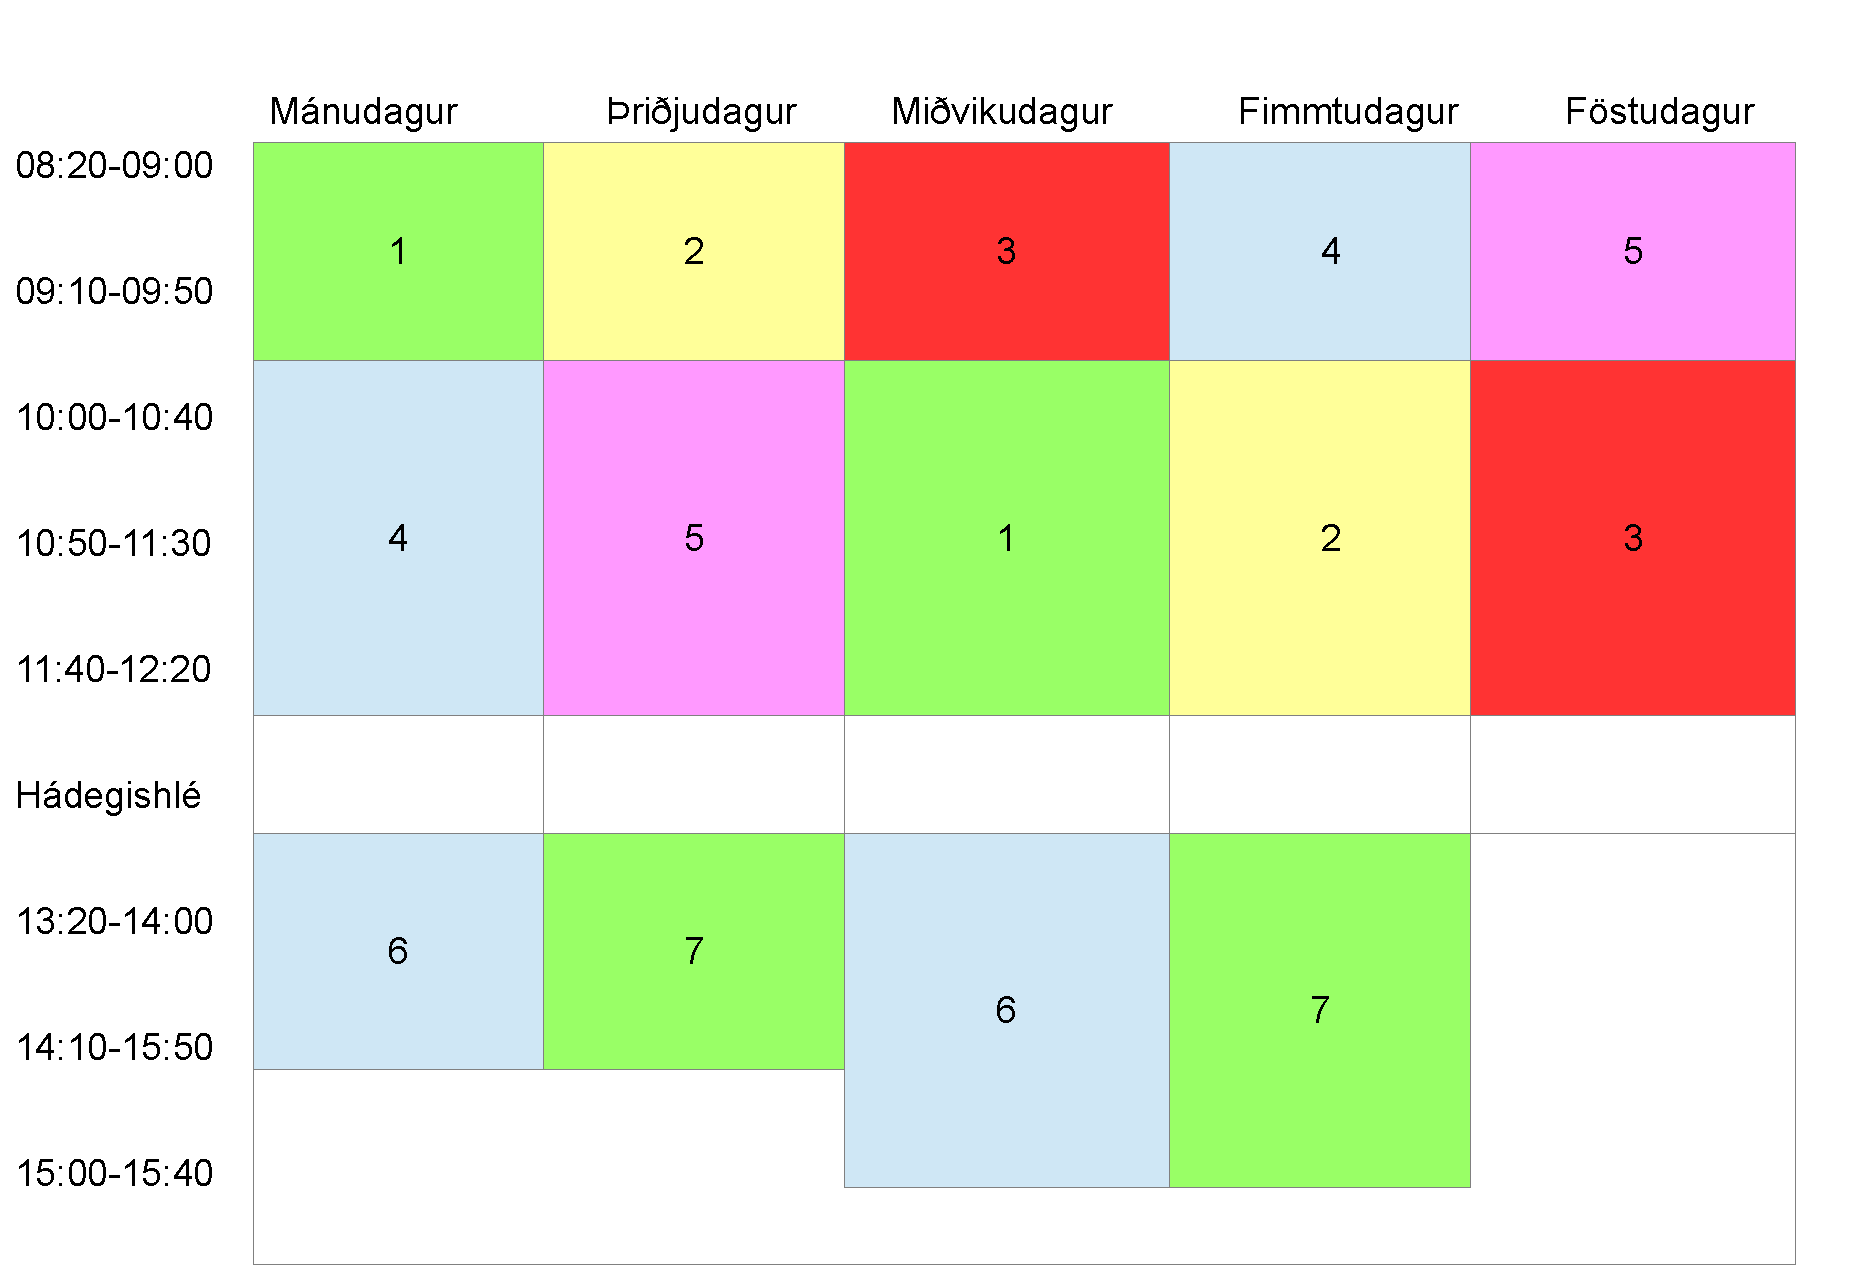
\includegraphics[scale=0.3]{stundatafla}
\end{center}

\begin{itemize}
\item Inngangur og markmið
\item Samantekt á uppgötvun og niðurstöðum
\item Samantekt á tillögum (má vitna í meginhluta skýrslu)
\end{itemize}


\section{Inngangur/bakgrunnur}


2 siður af rugli





\section{Niðurstöður, niðurlag og tillögur}
\begin{itemize}
\item Aðalniðurstöður
	

\item Aukaniðurstöður → Viðauka
\item Yfirgripsmikil gögn eða greining
\item Stuðningsniðurstöður → Viðauka
\end{itemize}

\textbf{a) } Byrjuðum á því að setja þá skorðu að hvert námskeið sé kennt aðeins einu sinni og hver stokkur taki að hámarki 5 kennslustundum samtals nema stokkur 8 sem getur tekið við afgangstímum. Pössuðum upp á að eitt námskeið við námskeiðshóp væri kennt í einu svo nemendur í þeim hópum lentu ekki í árekstrum. Lögleg lausn fannst á þessu keyrsluforriti.

Markfalli var svo bætt við sem hámarkaði fjölda námskeiða í stokki 1-5 og lágmarkaði þá sem lenda utan stokka.\\
\textbf{b)} \\
\lstinputlisting{stundatoflugerd.mod}

\textbf{c)} tölfræði árekstra, hvers eðlis eru árekstrarnir fyrir Eðlisfræðina, núverandi stundatöflur fyrir vormisseri, bæta við fleiri námskeiðshópum?......bæta við og leysa aftur

\begin{center}
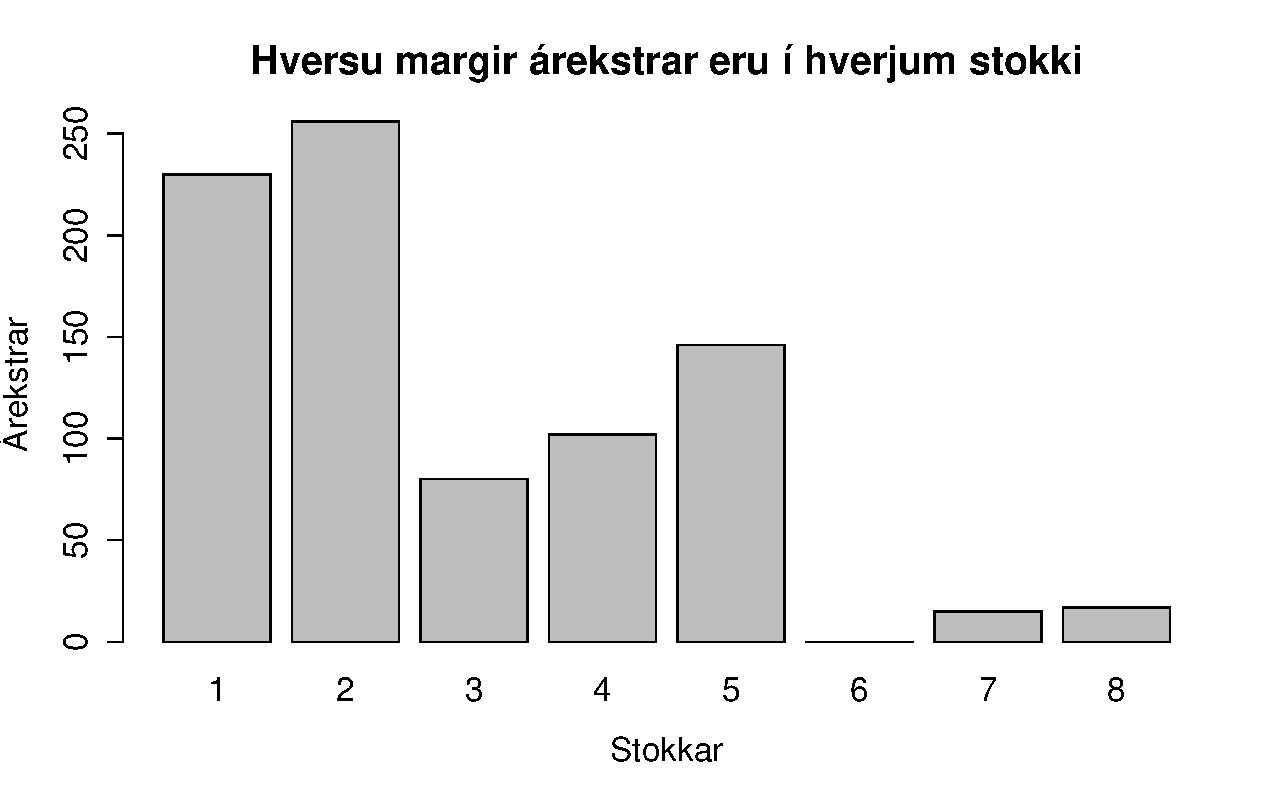
\includegraphics[scale=0.5]{c_lidur_plot}
\end{center}
d)koma námskeiðum fyrir í NamskeidStokkur, hversu vel er hægt að uppfylla


e)kennslustofunýting, námskeið fyrir hádegi


f)besta útfærsla stundatöflu....heildarfjöldi árekstra

\section{Aðferðir}
frásögn þannig að annar nemandi skilji það og að aðrir geti í
grundval laratriðum endurtekið niðurstöðurnar
\begin{itemize}
\item Fræði
\item Tækni
\item Greining
\item Reiknirit
\end{itemize}


Almennt línulegt bestunarlíkan er þar sem gefið er:

Hráefni(e.resources) með takmörkuðu framboði $b_i$, á hráefni i þar sem:
\[i=1,....,m\]
Framleiðsluvörur(e.activities), ákvarðað er $x_j$ sem er framleitt magn eininga af vöru j þar sem:
\[j=1,....,m\]
Hagnaður $c_j$ af hverri einingu j. 

Notkun hráefnis i í vöru j þar sem $a_{ij}$.

Verkefnið er að hámarka(eða lágmarka):
\[max_{x1,.....,xn}Z = \sum_{j=1}^{n}c_j x_j\]
með skorðum i=1,...,m.
\[\sum_{j=1}^{n}a_{ij} x_j\leq b_i\]
\[x_j\geq 0, j=1,....,n\]
Fylkjaform:
\[max_xZ=c^Tx\]
með skorðum:
\[Ax\leq b\]
\[x\geq 0\]

\section{Almenn umfjöllun....sleppa??}
\begin{itemize}
\item Skyld verkefni
\item Skyld rit
\item Aðrar leiðir sem hafa ekki verið prófaðar
\end{itemize}




\pagebreak
\section{Heimildir}



\pagebreak
\section{Viðauki}
má setja á tölvudisk með góðum útskýringum
\begin{itemize}
\item Stærðfræðileg líkön
\item Flæðirit
\item Gögn
\item Stórar töflur með niðurstöðum
\end{itemize}

\end{document}


